\documentclass[12pt]{article} % Se vuoi scrivere in 14pt la classe dovrà essere 'extarticle'

% Pacchetti base
\usepackage[T1]{fontenc} % Codifica dei font: fornisce a LaTeX i caratteri accentati e altra roba di questo tipo
\usepackage[utf8]{inputenc} % Serve a LaTeX per interpretare correttamente i caratteri immessi nell'editor (utf8 oppure latin1)
\usepackage{ulem}
\usepackage[greek.ancient,italian]{babel} % Lingue del documento, l'ultima è quella principale
\newcommand{\greco}{\foreignlanguage{greek}}
\addto\captionsitalian{\renewcommand{\abstractname}{Abstract}} % Per fare in modo che l'abstract venga nominato come "Abstract" e non come "Sommario"



% Formattazione generale
\usepackage{lmodern} % Il font usato sarà il Latin Modern (migliore nel posizionamento degli accenti rispetto a CModern)
\usepackage{helvet} % Pone l'Helvetica come font default per lo stile sans-serif
%\renewcommand{\familydefault}{\sfdefault} % Rende il sans-serif lo stile di default per il documento (eccetto che per la matematica)
\usepackage{microtype} % Pacchetto-boss per la microtipografia
\usepackage{indentfirst} % Produce il rientro della prima riga del primo capoverso di una sezione (Einaudi fa così XD)
%\setlength\parindent{0pt} % Elimina il rientro della prima riga di ogni capoverso
%\usepackage{layaureo} % Allarga un po' i margini rispetto allo standard, senza però allargarli troppo (discreta leggibilità) e mettendo larghezza e altezza del testo in sezione aurea
\usepackage{geometry} % Imposta i margini della pagina (continua riga sotto).
\geometry{a4paper,top=2cm,bottom=2cm,left=1.5cm,right=1.5cm,heightrounded} % Per aggiungere uno spazio di rilegatura piazzi alla fine 'bindingoffset= x mm'. Le dimensioni standard di Word sono 'top=2.5cm,bottom=2cm,left=2cm,right=2cm'. Per impostare tutte le pagine del documento in orizzontale inserisci anche l'opzione 'landscape'
\usepackage{enumitem} % Regola la spaziatura degli elenchi (continua sotto)
%\setlist{topsep=0.85em,parsep=0.45em,itemsep=0.1em} % 'topsep' regola la spaziatura fra i paragrafi prima e dopo l'ambiente, 'parsep' regola la spaziatura fra i paragrafi di uno stesso \item, 'itemsep' regola la spaziatura fra gli \item
\setdescription{labelindent=0em,labelsep=1em,leftmargin=\parindent} % 'labelindent' è la distanza del contrassegno dal margine della pagina, messa a 0 perché tutto il documento è un grande elenco quindi è inutile indentare | 'leftmargin' è l'indentazione delle righe successive alla prima in una voce, messa uguale a \parindent perché così è come se fosse un testo scritto normale | 'labelsep' è la distanza fra il contrassegno dal resto del testo nella prima riga di ogni voce

% Colori
\usepackage[svgnames,table,xcdraw]{xcolor} % Pacchetto che fornisce i colori, [svgnames] aumentare il database di colori disponibili
% Colori svgnames: Navy è più saturo di MidnightBlue
% \definecolor{jeans}{RGB}{0,42,84} % Definisce un colore che poi puoi usare altrove nel documento; prima il nome, poi il modello di colore (RGB è diverso da rgb) e poi la definizione del colore

% Figure e tabelle
\usepackage{graphicx} % Per inserire file esterni in figure
\usepackage{subfig} % Permette di inserire più figure all'interno dello stesso oggetto mobile
\usepackage{float} % Scrivendo [H] nelle preferenze di collocazione di un oggetto mobile, te lo mette proprio dove l'hai inserito.
\usepackage{wrapfig} % Per inserire figure "immerse" nel testo
\usepackage{booktabs} % Per produrre i filetti delle tabelle
\usepackage{caption} % Per produrre le didascalie (continua sotto)
\captionsetup{labelfont={sf,bf},tableposition=top,figureposition=bottom,font=small} % Specifiche per le didascalie: 'format=hang' allinea alla prima riga quelle successive | 'labelfont={sf,bf}' imposta l'etichetta della didascalia in caratteri senza grazie neri | specifica dove mettere la didascalia: sopra per le tabelle, sotto per le figure
\usepackage{floatflt,epsfig}
% Pacchetti scientifici
\usepackage[detect-all,output-decimal-marker={,},list-pair-separator={ e },list-final-separator={ e },range-units=single,range-phrase={--}]{siunitx} % Scrive correttamente le unità di misura SI: detect-all fa in modo che le unità di misura siano scritte riconoscendo le indicazioni di stile come grassetto e font serif/sans serif | output-decimal-marker specifica che il delimitatore decimale sia la virgola e non il punto | list-pair-separator specifica che il separatore fra due grandezze sia la 'e' | list-final-separator specifica che il separatore dell'grandezza sia la 'e' | range-phrase specifica il separatore fra la prima e la seconda grandezza | [retain-explicit-plus], che è meglio usare localmente, tiene esplicito il + di una grandezza
\usepackage{chemformula} % Per comporre formule chimiche
\usepackage{amsmath} % Pacchetto di estensioni per comporre la matematic
\usepackage{mathtools}
\usepackage{amssymb} % Rende disponibili una serie di simboli utili in matematica; carica automaticamente anche 'amsfonts'
% TikZ
\usepackage{tikz}

% Riquadri colorati tcolorbox
\usepackage{tcolorbox}
\newtcolorbox{riquadrostandard}[1]{colback=red!5!white,colframe=red!75!black,fonttitle=\bfseries,title=#1}
\newtcolorbox{regola}[1]{width=0.80\linewidth,colback=red!5,colframe=red!42,coltitle=black,halign title=center,fonttitle=\bfseries\large,title=#1}

% Bibliografia automatica
%\usepackage[hyperref=true,style=authoryear-comp]{biblatex} % Pacchetto per la bibliografia con le opzioni
%\addbibresource{Bibliografia-.bib} % Specifica da quale file prendere le referenze bibliografiche
% Altri pacchetti
\usepackage{footnotebackref} % Rende cliccabili le note a piè di pagina in modo che portino alla posizione nel testo a cui si riferiscono
\usepackage{pdfpages} % Per inserire pagine di un pdf esterno. Nel corpo del documento scrivi \includepdf[pages=2,3,5-8]{nome_pdf}; in base a dove metti il comando lui inizia una nuova pagina inserendo il pdf e quando ha finito riparte con una nuova pagina. Di default inserisce solo la pagina 1
\usepackage[font=small]{quoting} % Per inserire ambienti testuali come quello di abstract all'inizio; li invochi con i soliti \begin{quoting} ed \end{quoting}
\usepackage{comment} % Per inserire commenti lunghi
\usepackage{lipsum} % Genera testo fittizio
\hyphenation{} % Regola la sillabazione (se devi regolare più parole separale con uno spazio). Se vuoi regolare la sillabazione di una parola solo in un punto del documento, inserisci dentro \mbox{testo} ciò che non vuoi separare

% Nuovi comandi
\newcommand{\zariv}[1]{\colorbox{Yellow}{\textcolor{Magenta}{D@RiV}}}
\newcommand{\wariv}[1]{\colorbox{Yellow}{.}}
%\newcommand{nome_comando}[1]{come_deve_apparire} % Nuovo comando, insomma la cosa del libro di botanica. Con {nome_comando} assegni il nome che scriverai nel sorgente ogni volta che vuoi richiamare il comando, con {come_deve_apparire} dici cosa vuoi che LaTeX scriva ogni volta che piazzi il comando. Per esempio: \newcommand{\pianta}[1]{\textit{#1}}

% Interlinea
%\usepackage{setspace} % Regola l'interlinea, vedi sotto
%\singlespacing \onehalfspacing \doublespacing % Per interlinea 1, 1,5 e 2
%\renewcommand{\baselinestretch}{1.3} % Da usare solo per frontespizi o cose particolari! Aumenta la spaziatura di TUTTO, quindi usa solo per documenti ad una pagina e poco altro. Il valore 1.25 è CIRCA uguale a quello che ottieni con '\onehalfspacing'

% Spazio per pacchetti/comandi temporanei
\usepackage{multicol}
\usepackage{pdfpages}
% Altro
%\pdfminorversion='x' % Di default LaTeX produce un PDF versione 1.5, se vuoi fare in modo che produca versioni precedenti o successive sostituisci ad 'x' la seconda cifa della versione (per esempio 7 per PDF 1.7)
\overfullrule=3em % Stampa un quadrato nero accanto alle righe che sporgono dal margine in modo da segnalare che sono state composte male
\usepackage{hyperref} % Pacchetto-boss per i collegamenti ipertestuali e i metadati del pdf; caricalo per ultimo (ma prima di bookmarks)
\hypersetup{
	pdftitle={Esercitazione Metodi Numerici per l'Ambiente Marco Falda },
	pdfauthor={Marco Falda},
	pdfsubject={ Metodi Numerici per l'Ambiente},
	pdfkeywords={},
	colorlinks=true,
	linkcolor=MidnightBlue, % colore del collegamento \ref{} che porta all'elemento ipertestuale segnato con \label{}
	citecolor=Brown, % colore del collegamento \cite{} che porta all'elemento citato in bibliografia con \bibitem{}
	urlcolor=DarkRed, % colore del collegamento \url{} ad una pagina web
	% hidelinks % lo piazzi se vuoi che i collegamenti ipertestuali vengano neri come il testo normale
}
\usepackage{bookmark} % Produce l'indice nel pdf e permette di personalizzarlo meglio rispetto al solo hyperref

\begin{document}
	%\pagenumbering{gobble} % Per non non far comparire i numeri di pagina
	%\renewcommand{\abstractname}{\vspace{-\baselineskip}} % Se vuoi scrivere un abstract/sommario senza che ti esca la scritta abstract/sommario
	
\begin{comment}
NOTE
	- *pezza finché non trovo il modo di inserire gli accenti giusti da tastiera* : `` servono per fare le virgolette ALL'INIZIO DI PAROLA, '' servono per fare le virgolette ALLA FINE DI PAROLA
	oppure “”
	- La tilde ~, messa fra due parole senza spazio indica che non le si vuole separare da un "fine riga a capo". Però si accetta che possano essere separate dal trattino di sillabazione di fine riga
\end{comment}

% INSERIRE IL CODICE SOTTOSTANTE SUBITO DOPO \begin{document} NEL DOCUMENTO DELLA RELAZIONE
\thispagestyle{empty} % Per non non far comparire il numero di pagina
\newgeometry{top=2.5cm,bottom=2cm,left=1cm,right=1cm,heightrounded}
{\linespread{2.3}\selectfont
{\sffamily
	\begin{figure}
		\centering
		
\includegraphics[width=0.75\textwidth]{logounitrento2019.jpg}
	\end{figure}
		
	\vspace*{-1.5em}
		
	\begin{center}
		{\Large Corso di Laurea Magistrale}\\
		\vspace*{-0.8em}
		{\Large in Ingegneria per l'Ambiente e il Territorio}\\
		\vspace*{0.5em}
		{\Large A.A. 2019/2020}
				
		\vspace*{4em}
		
		{\Huge \textbf{Idrodinamica}}\\{\Large Esercitazione Numerica III}
		
		\vspace*{4em}
		
		{\Large Prof. Dr. Ing. Marco Tubino}
	\end{center}
	
	\vspace*{3.2em}
	
	\begin{center}
	\begin{multicols}{2}
	\begin{flushright}
	{\Large
		Studente: Marco Falda\\
%		Matricola:\\
		%Data:\\
	}
	\end{flushright}
	\begin{flushleft}
	{\Large
%		Studente:\\
		\hspace*{1em}Matricola: 213754\\
		%11/11/2019
	}
	\end{flushleft}
	\end{multicols}
	\end{center}

}
}
\restoregeometry

\newpage
\thispagestyle{empty}
\tableofcontents

\newpage
\listoffigures

\newpage
\section{Obiettivi}
\noindent Scopo dell’esercitazione è lo studio dei processi fluidodinamici di moto vario tramite l’analisi di due fenomeni caratterizzati da scale temporali diverse, in particolare la rottura di una diga (evento rapido) e il passaggio di un’onda di piena (evento lento).
L’evoluzione temporale dei fenomeni viene analizzata tramite opportuni schemi numerici di risoluzione, implementati per mezzo di un codice in linguaggio Python.
Si considera in partenza l’ipotesi di corrente non stazionaria, cioè con variazioni riscontrabili nel tempo.

\newpage
\section{Introduzione}
\subsection{I modelli idrodinamici unidimensionali: il modello di corrente}
\noindent 
Nello studio dei fenomeni di moto vario, il livello di elaborazione del modello utilizzato dipende dal grado di complessità del fenomeno trattato, sulla base del quale i modelli idrodinamici vengono classificati in:
\begin{itemize}
    \item Modelli tridimensionali (circolazioni oceaniche, laghi, turbolenza)
    \item Modelli bidimensionali (confluenze, biforcazioni, dinamiche di esondazione)
    \item Modelli unidimensionali (propagazione di onde di piena)
    \item Modelli zero-dimensionali (riempimento e svuotamento di serbatoi).
\end{itemize}
\noindent Nel caso in esame, il modello unidimensionale di corrente offre una descrizione sufficientemente accurata della variazione delle grandezze caratteristiche, ovvero velocità, quantità di moto ed energia, la quale avviene preferibilmente lungo un’unica direzione. Le componenti trasversali sono infatti trascurabili, dal momento che subiscono variazioni di diversi ordini di grandezza minori.
\\
Nel modello di corrente si considera una sola coordinata spaziale oltre a quella temporale. Le variabili indipendenti saranno pertanto ridotte a due: x e t.
\\
Si definiscono sezioni le intersezioni della corrente con i piani ortogonali alla direzione prevalente delle linee di corrente, in generale non rettilinee. La corrente è descritta per mezzo di quantità dinamiche (velocità, quantità di moto) ed energetiche (energia) localmente mediate sulla sezione. \\
Il modello di corrente può essere applicato qualora sussistano le seguenti ipotesi:
\begin{itemize}
    \item la curvatura della linea d’asse è sufficientemente piccola ed i moti secondari sono modesti, tali da non contraddire l’esistenza di una direzione prevalente del moto
    \item le variazioni spazio-temporali della forma della sezione sono sufficientemente lente, tali da non contraddire il vincolo di quasi unidirezionalità del moto
    \item la velocità verticale è significativamente più piccola rispetto alla velocità orizzontale (condizione verificata nell’ipotesi di bassa profondità)
    \item la velocità trasversale è significativamente più piccola rispetto a quella nella direzione prevalente del moto
    \item la superficie libera si può assumere orizzontale nella direzione trasversale (si trascurano le variazioni trasversali del carico piezometrico)
\end{itemize}

\subsection{Le equazioni delle correnti di De Saint-Venant}
\noindent Le equazioni differenziali che governano il moto delle correnti a superficie libera sono il principio di conservazione della massa:
\begin{equation}
    \frac{\partial \Omega }{\partial t}+\frac{\partial Q}{\partial x}=0
    \label{eqn:cons_massa}
\end{equation}
\noindent ed il principio di conservazione della quantità di moto:
\begin{equation}
    \frac{\partial Q }{\partial t}+\frac{\partial}{\partial x}\left(\beta\frac{Q^2}{\Omega}\right)+g\Omega\frac{\partial h}{\partial x}+\frac{\tau_0p}{\rho}=0
    \label{eqn:cons_q_moto}
\end{equation}

\newpage

\noindent dove:
\begin{itemize}
    \item $\Omega$ è la sezione dell'alveo [$m^2$]
     \item $Q$ è la portata [$m^{2}\cdot s^{-1}$]
    \item $\beta$ è il coefficiente di ragguaglio della quantità di moto [$adm$]
    \item g è l'accelerazione gravitazionale [$m\cdot s^{-2}$]
    \item $h$ è la quota della superficie libera [$m$]
    \item $\tau_0$ è lo sforzo tangenziale al fondo [$kg\cdot m^{-1}\cdot s^{-2}$]
    \item $p$ è il perimetro bagnato [$m$]
    \item $\rho$ è la densità dell’acqua [$kg\cdot m^{-3}$]
\end{itemize}
\noindent Ai fini dell'esercitazione, si assume che l'alveo sia cilindrico ($\beta$ = 1):
\begin{equation}
    \frac{\partial Q }{\partial t}+\frac{\partial}{\partial x}\left(\frac{Q^2}{\Omega}\right)+g\Omega\frac{\partial h}{\partial x}+\frac{\tau_0p}{\rho}=0
    \label{eqn:cons_q_moto_cil}
\end{equation}
\noindent Il problema del moto si traduce quindi nella risoluzione di un sistema a due equazioni, (\ref{eqn:cons_massa}) e (\ref{eqn:cons_q_moto_cil}), rispetto a tre incognite, $\Omega(x,t)$, $Q(x,t)$ e $\tau_0(x,t)$. Dal momento che il numero di incognite è sovrabbondante rispetto al numero di equazioni, è necessario introdurre una relazione di chiusura:
\begin{equation}
    \tau_0 = \rho\frac{u^{2}}{C^{2}}
    \label{eqn:chiusura}
\end{equation}
dove:
\begin{itemize}
\item $u$ è la velocità mediata sulla profondità [$m\cdot s^{-1}$]
\item C è detta conduttanza [$adm$]
\end{itemize}
e dove $C^2$ è uguale a:  
\begin{equation}
    C^2=\frac{u^2}{gR_ij}
    \label{eqn:Chezy}
\end{equation}
\noindent Detta anche formula di Chezy, dove:
\begin{itemize}
    \item $R_i$ è il raggio idraulico [$m$]
    \item $j$ è un termine dissipativo che rappresenta la perdita di carico dovuta all'attrito [$adm$]
\end{itemize}
\noindent Sostituendo (\ref{eqn:Chezy}) in (\ref{eqn:chiusura}) ricaviamo un'espressione per la tensione al fondo:
\begin{equation}
    \tau_0=\rho gR_ij
    \label{eqn:tensione_fondo}
\end{equation}
\noindent Sostituendo $\tau_0$ in (\ref{eqn:cons_q_moto_cil}) otteniamo finalmente:
\begin{equation}
    \frac{\partial Q }{\partial t}+\frac{\partial}{\partial x}\left(\frac{Q^2}{\Omega}\right)+g\Omega\frac{\partial h}{\partial x}+{g\Omega j}=0
    \label{eqn:cons_q_moto_chius}
\end{equation}
\subsubsection{Forma conservativa}
\noindent Assumendo ancora, ai fini dell'esercizio, che l'alveo sia rettangolare, le equazioni delle correnti possono essere anche espresse nella forma conservativa come:
\begin{equation}
    \frac{\partial \Omega }{\partial t}+\frac{\partial Q}{\partial x}=0
    \label{eqn:cons_massa_cons}
\end{equation}
\begin{equation}
    \frac{\partial Q }{\partial t}+\frac{\partial}{\partial x}\left(\frac{Q^2}{\Omega}+g\frac{\Omega^2}{2B}\right)={g\Omega\left(i_F-j\right)}
    \label{eqn:cons_q_moto_cons}
\end{equation}
\noindent dove:
\begin{itemize}
    \item $i_F$ è la pendenza del fondo [$adm$]
    \item $B$ è la larghezza dell'alveo [$m$]
\end{itemize}
\noindent Infatti, ricordando che:
\begin{equation}
    h=Y+z_F
    \label{eqn:h}
\end{equation}
\noindent dove:
\begin{itemize}
    \item $Y$ è il tirante idraulico [$m$]
    \item $z_F$ è la quota del fondo [$m$]
\end{itemize}
\noindent da cui:
\begin{equation}
    \frac{\partial h}{\partial x}=\frac{\partial }{\partial x}\left(Y+z_F\right)=\left(\frac{\partial Y}{\partial x}-i_F\right)
    \label{eqn:dh/dx}
\end{equation}
\noindent possiamo riscrivere (\ref{eqn:cons_q_moto_chius}) come:
\begin{equation*}
    \frac{\partial Q }{\partial t}+\frac{\partial}{\partial x}\left(\frac{Q^2}{\Omega}\right)+g\Omega\left(\frac{\partial Y}{\partial x}-i_F\right)+{g\Omega j}=0
\end{equation*}
\begin{equation}
    \frac{\partial Q }{\partial t}+\frac{\partial}{\partial x}\left(\frac{Q^2}{\Omega}\right)+g\Omega\frac{\partial Y}{\partial x}=g\Omega\left(i_F-j\right)
       \label{eqn:cons_q_moto_iF}
\end{equation}
\noindent Inoltre, essendo per ipotesi l'alveo rettangolare:
\begin{equation}
    \Omega=B Y
    \label{eqn:Omega}
\end{equation}
\noindent ed essendo $B$ costante (alveo prismatico, $\Omega = \Omega(Y)$):
\begin{equation}
    \frac{\partial \Omega}{\partial x}=\frac{\partial }{\partial x}\left(BY\right)=B\frac{\partial Y}{\partial x}
    \label{eqn:dOmega/dx}
\end{equation}
\noindent ne consegue che:
\begin{equation}
    \frac{\partial}{\partial x}\left(g\frac{\Omega^2}{2B}\right)=g\frac{\Omega}{B}\frac{\partial \Omega}{\partial x}=g\Omega\frac{\partial Y}{\partial x}
    \label{eqn:gOmegadY/dx}
\end{equation}
\noindent Sostituendo (\ref{eqn:gOmegadY/dx}) in (\ref{eqn:cons_q_moto_iF}) otteniamo (\ref{eqn:cons_q_moto_cons}), come volevasi dimostrare.\\
\noindent In notazione vettoriale, il sistema formato dalle equazioni (\ref{eqn:cons_massa_cons}) e (\ref{eqn:cons_q_moto_cons}) assume la seguente forma:
\begin{equation}
    \frac{\partial U}{\partial t}+\frac{\partial F}{\partial x}  = S(U)
    \label{eqn:forma_cons_vett}
\end{equation}
\noindent dove:
\begin{align*}
    U=\begin{vmatrix}\Omega\\Q\end{vmatrix} &&
    F=\begin{vmatrix}Q\\\frac{Q^2}{\Omega}+g\frac{\Omega^2}{2B}\end{vmatrix} &&
    S=\begin{vmatrix}0\\g\Omega(i_F-j)\end{vmatrix}
\end{align*}
\noindent Il termine $S(U)$ è detto termine sorgente. 
\subsubsection{Forma conservativa ridotta}
\noindent Trovandoci nelle condizioni di alveo cilindrico e rettangolare, possiamo semplificare il sistema (\ref{eqn:cons_massa_cons}), (\ref{eqn:cons_q_moto_cons}) dividendo entrambe le equazioni per la larghezza della superficie libera $B$, che è una costante. Otterremo perciò:
\begin{equation}
    \frac{\partial Y}{\partial t}+\frac{\partial q}{\partial x}=0
    \label{eqn:cons_massa_cons_rid}
\end{equation}
\begin{equation}
    \frac{\partial q }{\partial t}+\frac{\partial}{\partial x}\left(\frac{q^2}{Y}+g\frac{Y^2}{2}\right)={gY\left(i_F-j\right)}
    \label{eqn:cons_q_moto_cons_rid}
\end{equation}
dove:
\begin{itemize}
    \item $q$ è la portata per unità di larghezza [$m^2\cdot s^{-1}$]
\end{itemize}
\noindent In notazione vettoriale:
\begin{equation}
    \frac{\partial U}{\partial t}+\frac{\partial F}{\partial x}  = S(U)
    \label{eqn:forma_cons_rid_vett}
\end{equation}
\noindent dove:
\begin{align*}
    U=\begin{vmatrix}Y\\q\end{vmatrix} &&
    F=\begin{vmatrix}q\\\frac{q^2}{Y}+g\frac{Y^2}{2}\end{vmatrix} &&
    S=\begin{vmatrix}0\\gY(i_F-j)\end{vmatrix}
\end{align*}
\subsubsection{Forma quasi lineare}
\noindent Esplicitando la derivata rispetto ad x in (\ref{eqn:cons_q_moto_cons_rid}):
\begin{equation*}
    \frac{\partial q }{\partial t}+\left(\frac{2q}{Y}\frac{\partial q}{\partial x}-\frac{q^2}{Y^2}\frac{\partial Y}{\partial x}+gY\frac{\partial Y}{\partial x}\right)={gY\left(i_F-j\right)}
\end{equation*}
\begin{equation}
    \frac{\partial q }{\partial t}+\left(gY-\frac{q^2}{Y^2}\right)\frac{\partial Y}{\partial x}+\frac{2q}{Y}\frac{\partial q}{\partial x}={gY\left(i_F-j\right)}
    \label{eqn:cons_q_moto_quasi_lin}
\end{equation}
\noindent In notazione vettoriale:
\begin{equation}
    \frac{\partial U}{\partial t}+J_F(U)\frac{\partial U}{\partial x}  = S(U)
    \label{eqn:forma_quasi_lin_vett_jacob}
\end{equation}
\noindent dove:
\begin{align*}
    J_F(U) =\frac{\partial F}{\partial U} = \begin{vmatrix}\frac{\partial q}{\partial Y} && \frac{\partial q}{\partial q} \\ \frac{\partial }{\partial Y}\left(\frac{q^2}{Y}+g\frac{Y^2}{2}\right) && \frac{\partial }{\partial q}\left(\frac{q^2}{Y}+g\frac{Y^2}{2}\right)\end{vmatrix} = \begin{vmatrix}0 && 1 \\ -\frac{q^2}{Y^2}+gY && \frac{2q}{Y}\end{vmatrix} && \frac{\partial U}{\partial x}=\begin{vmatrix}\frac{\partial Y}{\partial x}\\\frac{\partial q}{\partial x}\end{vmatrix}
\end{align*}
\noindent Risultato che avremmo anche potuto ottenere applicando direttamente la regola della catena a (\ref{eqn:forma_cons_rid_vett}):
\begin{equation}
    \frac{\partial U}{\partial t}+\frac{\partial F}{\partial U}\frac{\partial U}{\partial x}  = S(U)
    \label{eqn:forma_quasi_lin_vett_catena}
\end{equation}
\noindent Le equazioni(\ref{eqn:cons_massa_cons_rid}) e (\ref{eqn:cons_q_moto_quasi_lin}) sono purtroppo equazioni differenziali non lineari (sono presenti infatti prodotti fra le incognite $Y$ e $q$), ma fortunatamente quasi-lineari (sono lineari rispetto alle derivate di $Y$ e $q$ di ordine massimo (Salsa S. 2016)). 

\subsubsection{Forma caratteristica}
\noindent Come abbiamo visto, in alcuni casi specifici le equazioni del flusso si riducono a sistemi di equazioni differenziali parziali del primo ordine quasi-lineari per due variabili indipendenti. Per tali sistemi può essere sviluppata una pressoché completa trattazione matematica, a patto che siano di natura iperbolica. Questa trattazione diventa particolarmente semplice quando il numero di funzioni ed equazioni è uguale a due (Courant R., Friedrichs K. O. 1977). \\
\noindent Sistemi di equazioni di questo tipo si presentano nella forma:
\begin{equation}
    \frac{\partial U_i}{\partial t}+J_{ik}\frac{\partial U_k}{\partial x}-S_i  = 0
    \label{eqn:sistema_iperbolico}
\end{equation}
\noindent dove:
\begin{itemize}
    \item $i$ rappresenta l'indice non ripetuto
    \item $k$ rappresenta l'indice ripetuto
\end{itemize}
\noindent Il problema più comune associato a tali sistemi è il seguente problema di valore iniziale (PVI): dati i valori della funzione sconosciuta al tempo $t=0$ $U(x,0)$, usare le equazioni per determinare l’evoluzione nel tempo della funzione $U(x,t)$ (Ben-Artzi M., Falcovitz J. 2003).\\
Al fine di conoscere il valore della funzione incognita nel punto $(x,t)$, possiamo provare a connettere il punto $(x,t)$ con il punto $(x_0,0)$ sull'asse $x$, portante il dato iniziale, mediante una curva $x=x(t)$ lungo la quale $U$ sia costante. Una curva di questo tipo prende il nome di curva caratteristica. Se poi il procedimento si può ripetere per ogni punto $(x,t)$ con  $x\in D \subseteq \mathbb{R}, t>0$, possiamo calcolare $ U$ in ogni punto ed il problema è risolto. Questo metodo è detto metodo delle caratteristiche (Salsa S. 2016).\\
L'idea è quella di assumere un atteggiamento lagrangiano. Si definisce innanzitutto la cosiddetta derivata materiale:
\begin{equation}
    \frac{D}{Dt}=\frac{\partial }{\partial t}+\left(u\cdot\nabla\right)
    \label{eqn:derivata_materiale_3D}
\end{equation}
\noindent dove:
\begin{itemize}
    \item $u$ è il vettore velocità del sistema di riferimento lagrangiano [$m\cdot s^{-1}$]
\end{itemize}
\noindent In una dimensione spaziale:
\begin{equation}
    \frac{d}{dt}=\frac{\partial }{\partial t}+\frac{dx}{dt}\frac{\partial }{\partial x}=\frac{\partial }{\partial t}+\lambda\frac{\partial }{\partial x}
    \label{eqn:derivata_materiale_1D}
\end{equation}
\noindent dove:
\begin{itemize}
    \item $\lambda=\frac{dx}{dt}$ rappresenta la velocità o celerità di propagazione di un fenomeno ondulatorio [$m\cdot s^{-1}$]
\end{itemize}
\noindent Ora, dal momento che moltiplicare per uno scalare ambo i membri di (\ref{eqn:sistema_iperbolico}) non invalida l'uguaglianza, possiamo chiederci se esistano degli scalari $l_i$ tali che:
\begin{equation}
    l_i\left(\frac{\partial U_i}{\partial t}+J_{ik}\frac{\partial U_k}{\partial x}-S_i\right)  = l_i\left(\frac{dU_i}{dt}-S_i\right)=0
    \label{eqn:sist_iperb_scal_1}
\end{equation}
\noindent In altre parole, possiamo chiederci se esistano degli scalari che ci permettano di trasformare un sistema di equazioni differenziali alle derivate parziali rispetto a due variabili indipendenti ($x$ e $t$) in un sistema di equazioni differenziali ordinarie, a patto che ci si muova lungo una traiettoria caratteristica ad una velocità $\lambda$.\\
\noindent Sviluppando infatti la derivata materiale:
\begin{equation}
    \frac{dU_i}{dt}=\frac{\partial U_i}{\partial t}+\frac{dx}{dt}\frac{\partial U_i}{\partial x}=\frac{\partial U_i}{\partial t}+\lambda\frac{\partial U_i}{\partial x}
    \label{eqn:derivata_materiale_Ui}
\end{equation}
\noindent sostituendo in (\ref{eqn:sist_iperb_scal_1}):
\begin{equation}
    l_i\left(\frac{\partial U_i}{\partial t}+J_{ik}\frac{\partial U_k}{\partial x}-S_i\right)  = l_i\left(\frac{\partial U_i}{\partial t}+\lambda\frac{\partial U_i}{\partial x}-S_i\right)
    \label{eqn:sist_iperb_scal_2}
\end{equation}
\noindent e semplificando:
\begin{equation}
    l_i\left(J_{ik}\frac{\partial U_k}{\partial x}\right)  = l_i\left(\lambda\frac{\partial U_i}{\partial x}\right)
    \label{eqn:sistema_eq_diff_ord}
\end{equation}
\noindent otteniamo effettivamente un sistema di equazioni differenziali ordinarie rispetto alla sola variabile $x$ (sempre che esista $l_i$).\\
\noindent Esplicitando le due equazioni:
\begin{equation}
    l_1\left(J_{11}\frac{\partial U_1}{\partial x}+J_{12}\frac{\partial U_2}{\partial x}\right) = l_1\left(\lambda\frac{\partial U_1}{\partial x}\right)
    \label{eqn:sistema_eq_diff_ord_1}
\end{equation}
\begin{equation}
    l_2\left(J_{21}\frac{\partial U_1}{\partial x}+J_{22}\frac{\partial U_2}{\partial x}\right) = l_2\left(\lambda\frac{\partial U_2}{\partial x}\right)
    \label{eqn:sistema_eq_diff_ord_2}
\end{equation}
\noindent e sommando ambo i membri a destra e sinistra dell'uguale di (\ref{eqn:sistema_eq_diff_ord_1}) e (\ref{eqn:sistema_eq_diff_ord_2}):
\begin{equation}
    l_1\left(J_{11}\frac{\partial U_1}{\partial x}+J_{12}\frac{\partial U_2}{\partial x}\right)+l_2\left(J_{21}\frac{\partial U_1}{\partial x}+J_{22}\frac{\partial U_2}{\partial x}\right) = \lambda\left(l_1\frac{\partial U_1}{\partial x}+l_2\frac{\partial U_2}{\partial x}\right)
\end{equation}
\noindent in notazione matriciale:
\begin{equation}
    \begin{vmatrix}l_1 \\ l_2\end{vmatrix}\cdot 
    \left(\begin{vmatrix}J_{11}&J_{12}\\J_{21}&J_{22}\end{vmatrix}\cdot\begin{vmatrix}U_1\\U_2\end{vmatrix}\right) = \lambda\begin{vmatrix}l_1 \\ l_2\end{vmatrix}\cdot\begin{vmatrix}U_1\\U_2\end{vmatrix}
    \label{eqn:sist_iperb_scal_matr}
\end{equation}
\noindent in forma compatta:
\begin{equation}
    l \cdot\left(J \cdot U\right)=\lambda\left(l \cdot U\right)
\end{equation}
\noindent Dal momento che uno scalare trasposto è uguale a se stesso:
\begin{equation}
    l \cdot\left(J \cdot U\right)=\left(l \cdot J \cdot U\right)^T=U \cdot J^T \cdot l
\end{equation}
\begin{equation}
    \lambda \left(l \cdot U\right)=\lambda \left(l \cdot U \right)^T=\lambda \left(U \cdot l \right)
\end{equation}
\noindent la (\ref{eqn:sist_iperb_scal_matr}) può essere riscritta come:
\begin{equation}
    \begin{vmatrix}U_1 \\ U_2\end{vmatrix}\cdot\left(
    \begin{vmatrix}J_{11}&J_{21}\\J_{12}&J_{22}\end{vmatrix}\cdot\begin{vmatrix}l_1\\l_2\end{vmatrix}\right) =\lambda\begin{vmatrix}U_1 \\ U_2\end{vmatrix}\cdot\begin{vmatrix}l_1\\l_2\end{vmatrix}
\end{equation}
\noindent Semplificando ambo i membri per $U$ perveniamo infine a:
\begin{equation}
    \begin{vmatrix}J_{11}&J_{21}\\J_{12}&J_{22}\end{vmatrix}\cdot\begin{vmatrix}l_1\\l_2\end{vmatrix} =\lambda\begin{vmatrix}l_1 \\ l_2\end{vmatrix}
    \label{eqn:problema_autovalori}
\end{equation}
\noindent che è un problema agli autovalori. L'autovalore $\lambda$ può essere individuato ponendo:
\begin{equation}
    det\left(J^T-\lambda I\right) = 0
    \label{eqn:determinante_uguale_zero}
\end{equation}
\noindent L'equazione caratteristica assume la forma:
\begin{equation}
    J_{11}J_{22}-\lambda(J_{11}+J_{22})+\lambda^2-J_{21}J_{12}
\end{equation}
\noindent equazione di secondo grado in $\lambda$, dove:
\begin{align*}
    &J_{11}=0 & &J_{12}=1 & &J_{21}-\frac{q^2}{Y^2}+gY & &J_{22}=\frac{2q}{Y}
\end{align*}
\noindent Sostituendo:
\begin{equation}
    \lambda^2-\frac{2q}{Y}\lambda -\left(gY-\frac{q^2}{Y^2}\right) = 0
\end{equation}
\begin{equation}
    \pm\lambda = \frac{q}{Y}\pm\sqrt{\left(\frac{q}{Y}\right)^2+\left(gY-\frac{q^2}{Y^2}\right)}=\frac{q}{Y}\pm\sqrt{gY}=u\pm\sqrt{gY}
\end{equation}
\noindent per qualsiasi alveo rettangolare cilindrico.\\
\noindent Lungo le traietorie $\lambda$, dette curve caratteristiche, il sistema (\ref{eqn:sistema_iperbolico}) si trasforma in un sistema alle derivate totali.
\noindent Ponendo ad esempio $l_2=1$ nella seconda riga di (\ref{eqn:problema_autovalori}):
\begin{equation}
    J_{12}l_1 + J_{22}=\lambda
\end{equation}
\begin{equation}
    l_1  =\frac{\lambda-J_{22}}{J_{12}}=\frac{\left(u\pm\sqrt{gY}\right)-2u}{1}=-u\pm\sqrt{gY} 
\end{equation}
\noindent e sostituendo i valori di $l_1$ e $l_2$ così trovati nel termine di destra dell'equazione (\ref{eqn:sist_iperb_scal_1}) si ottiene:
\begin{equation}
    \left(-u\pm\sqrt{gY}\right)\frac{dY}{dt}+\frac{dq}{dt}-gY\left(i_F-j\right)=0
    \label{eqn:forma_caratteristica}
\end{equation}

\subsection{Onde di piena}
\noindent Le onde di piena fanno parte della categoria dei fenomeni lenti, agenti su scale spaziali e temporali molto ampie, caratterizzate nella loro trattazione matematica da un termine frizionale dominante e un termine inerziali poco influente.  
\subsubsection{PVI}
\noindent Consideriamo ora il PVI costituito da un'equazione differenziale dalla forma (\ref{eqn:cons_q_moto_quasi_lin}) definita su di un dominio $D=[0,L]\times[0,t^{fin}]$ soggetta ad una condizione iniziale del tipo:
\begin{align}
    U(x,0) = U^o(x) && x \in [0,L]
\end{align}
\noindent dove $U^o(x)$ rappresenta lo stato iniziale di tirante e portata su tutto il dominio di calcolo.\\
\noindent Siano inoltre note le seguenti condizioni al contorno:
\begin{align}
    &U(0,t) = U_L(t) && t \in [0,t^{fin}]\\
    &U(L,t) = U_R(t) && t \in [0,t^{fin}]
\end{align}
\noindent dove:
\begin{itemize}
    \item $U_L(t)$ rappresenta la condizione al contorno imposta all'estremità sinistra del dominio D
    \item $U_R(t)$ rappresenta la condizione al contorno imposta all'estremità destra del dominio D
\end{itemize}
\noindent La definizione del vettore delle incognite $U$ agli estremi del dominio di integrazione per $t \geq 0$ assicura la possibilità di risolvere la (\ref{eqn:forma_cons_rid_vett}) su tutto il dominio spaziale e per ciascun istante temporale $t \geq 0$.

\subsection{Rottura di una diga}
\noindent Le dighe sono serbatoi artificiali che immagazzinano grandi volumi di acqua confinata da elevazioni naturali del terreno, come un canyon o una valle, e pareti artificiali. Tuttavia, sebbene abbiano comportato numerosi benefici per la società, come fonti di acqua per il consumo umano e per l'irrigazione, generazione di energia idroelettrica e controllo di piene, lungo gli anni le dighe sono state anche al centro di numerosi eventi catastrofici. Questi eventi possono essere la conseguenza diretta del crollo improvviso delle pareti della diga. Tali crolli possono a loro volta indurre un flusso d'acqua che causa devastazione lungo il suo cammino nelle valli, con danni considerevoli alle proprietà e perdita di vite umane . I processi che portano al collasso di una diga sono vari e estremamente complessi. Come parte dell'analisi del rischio per la protezione civile, devono essere prodotte mappe di inondazione. Queste sono attualmente basate sulla simulazione numerica delle onde di propagazione. Le equazioni su acqua bassa dipendenti dal tempo, a una o due dimensioni spaziali, sono normalmente accettate come modello matematico base per studiare i fenomeni di propagazione delle onde indotti da eventi di collasso di una diga (Toro E. F. 2001).

\begin{figure} [H]
    \centering
    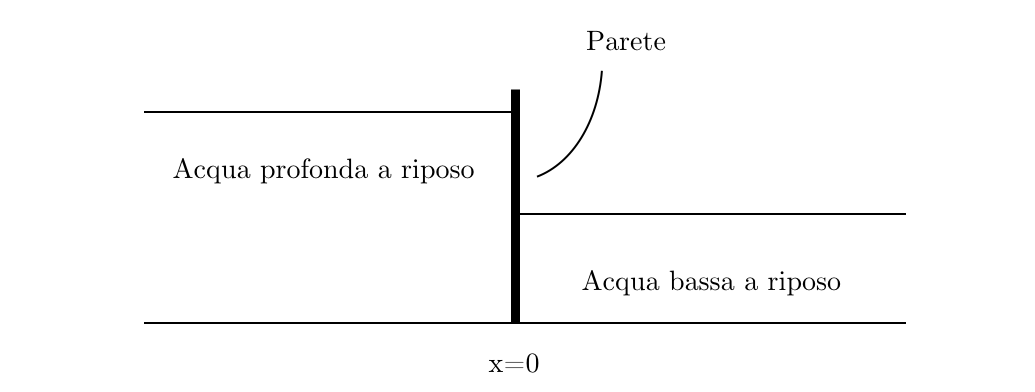
\includegraphics[width=0.6\columnwidth]{Dam Break.png}
    \caption{Condizioni iniziali nel problema di rottura di una diga. Una parete separa due livelli costanti di acqua a riposo.}
    \label{fig:Dam Break}
\end{figure}

\subsubsection{Modello 1D}
\noindent Si immagini un canale orizzontale di sezione rettangolare uniforme. Si supponga inoltre che il canale presenti due livelli costanti di pelo libero, entrambi a riposo, separati da un muro alla posizione $x=0$ (Figura \ref{fig:Dam Break}).
\noindent Se la parete che separa i due livelli costanti collassa, due caratteristiche dominanti emergono dal processo nella forma di onde. Un'onda rivolta verso destra viaggia nella porzione poco profonda del fluido, aumentando la profondità \textit{ex abrupto}. L'onda rivolta verso sinistra viaggia nella regione di acqua profonda e ha l'effetto di ridurre l'altezza del pelo libero. Se la parete collassa in un tempo sufficientemente piccolo, il modello ondulatorio che emerge è quasi quello di un sistema ondulatorio centrato con un'onda di rarefazione a sinistra ed un'onda di shock a destra; tali sistemi ondulatori possono essere approssimati dalle equazioni su acqua bassa (Toro E. F. 2001).
\subsubsection{PVI}
\noindent Una generalizzazione per le equazioni su acqua bassa del problema della rottura di una diga è il cosiddetto problema di Riemann. Formalmente, il problema di Riemann è definito come il seguente problema ai valori iniziali (Toro E. F. 2001):
\begin{equation}
    \frac{\partial U}{\partial t}+\frac{\partial F(U)}{\partial x}=0
    \label{eqn:Riemann}
\end{equation}
\begin{equation}
    U(x,0)=\begin{cases}U_L\quad se\quad x<0\\
    U_R\quad se\quad x>0
    \end{cases}
    \label{eqn:Riemann_cond_iniziali}
\end{equation}
\noindent dove $U_L$ e $U_R$ sono vettori costanti e rappresentano le condizioni iniziali al tempo $t=0$, rispettivamente a sinistra e a destra della coordinata $x=0$.
\newpage
\section{Metodologia}
\subsection{Metodi numerici adottati}
\subsubsection{Metodi numerici conservativi}
\noindent Si consideri il sistema unidimensionale di leggi di conservazione (\ref{eqn:Riemann}). Questa è chiamata forma differenziale delle leggi di conservazione ed è valida soltanto per il caso in cui la soluzione è regolare su tutto il dominio. Nella presenza di discontinuità, dev'essere usata la formulazione integrale (Toro E. F. 2001).
\noindent Applichiamo ora il Teorema di Green (Pagani C. D., Salsa S. 2016)
\begin{equation}
    \oint f(x,t)dx + g(x,t)dt = \iint \left(\frac{\partial g}{\partial x}-\frac{\partial f}{\partial t}\right)dxdt
    \label{eqn:teorema_Green}
\end{equation}
\noindent a (\ref{eqn:Riemann}), con $f(x,t) = -U(x,t)$ e $g(x,t) = F(x,t)$:
\begin{equation}
    \iint \left(\frac{\partial U}{\partial t}+\frac{\partial F}{\partial x}\right)dxdt = \oint F(x,t)dt - U(x,t)dx = 0
    \label{eqn:teorema_Green_app_Riemann}
\end{equation}
\noindent dove l'integrale di linea è calcolato lungo il contorno del dominio in senso antiorario. La risoluzione del sistema omogeno (\ref{eqn:Riemann}) si riassume quindi nella determinazione del valore che assume l'integrale di due funzioni vettoriali, $F(x,t)$ e $U(x,t)$, quando calcolato lungo una qualsiasi linea chiusa. 
\subsubsection{Metodo ai volumi finiti}
\noindent Si consideri a questo proposito un generico volume di controllo $V^{i}_n$ nel piano $(x,t)$ di forma rettangolare (Figura \ref{fig:Volume di controllo}), definito come: 
\begin{equation}
    V^{n}_i=[x_{i-\frac{1}{2}},x_{i+\frac{1}{2}}]\times[t^n,t^{n+1}]
    \label{eqn:volume_di_controllo}
\end{equation}
\begin{figure} [H]
    \centering
    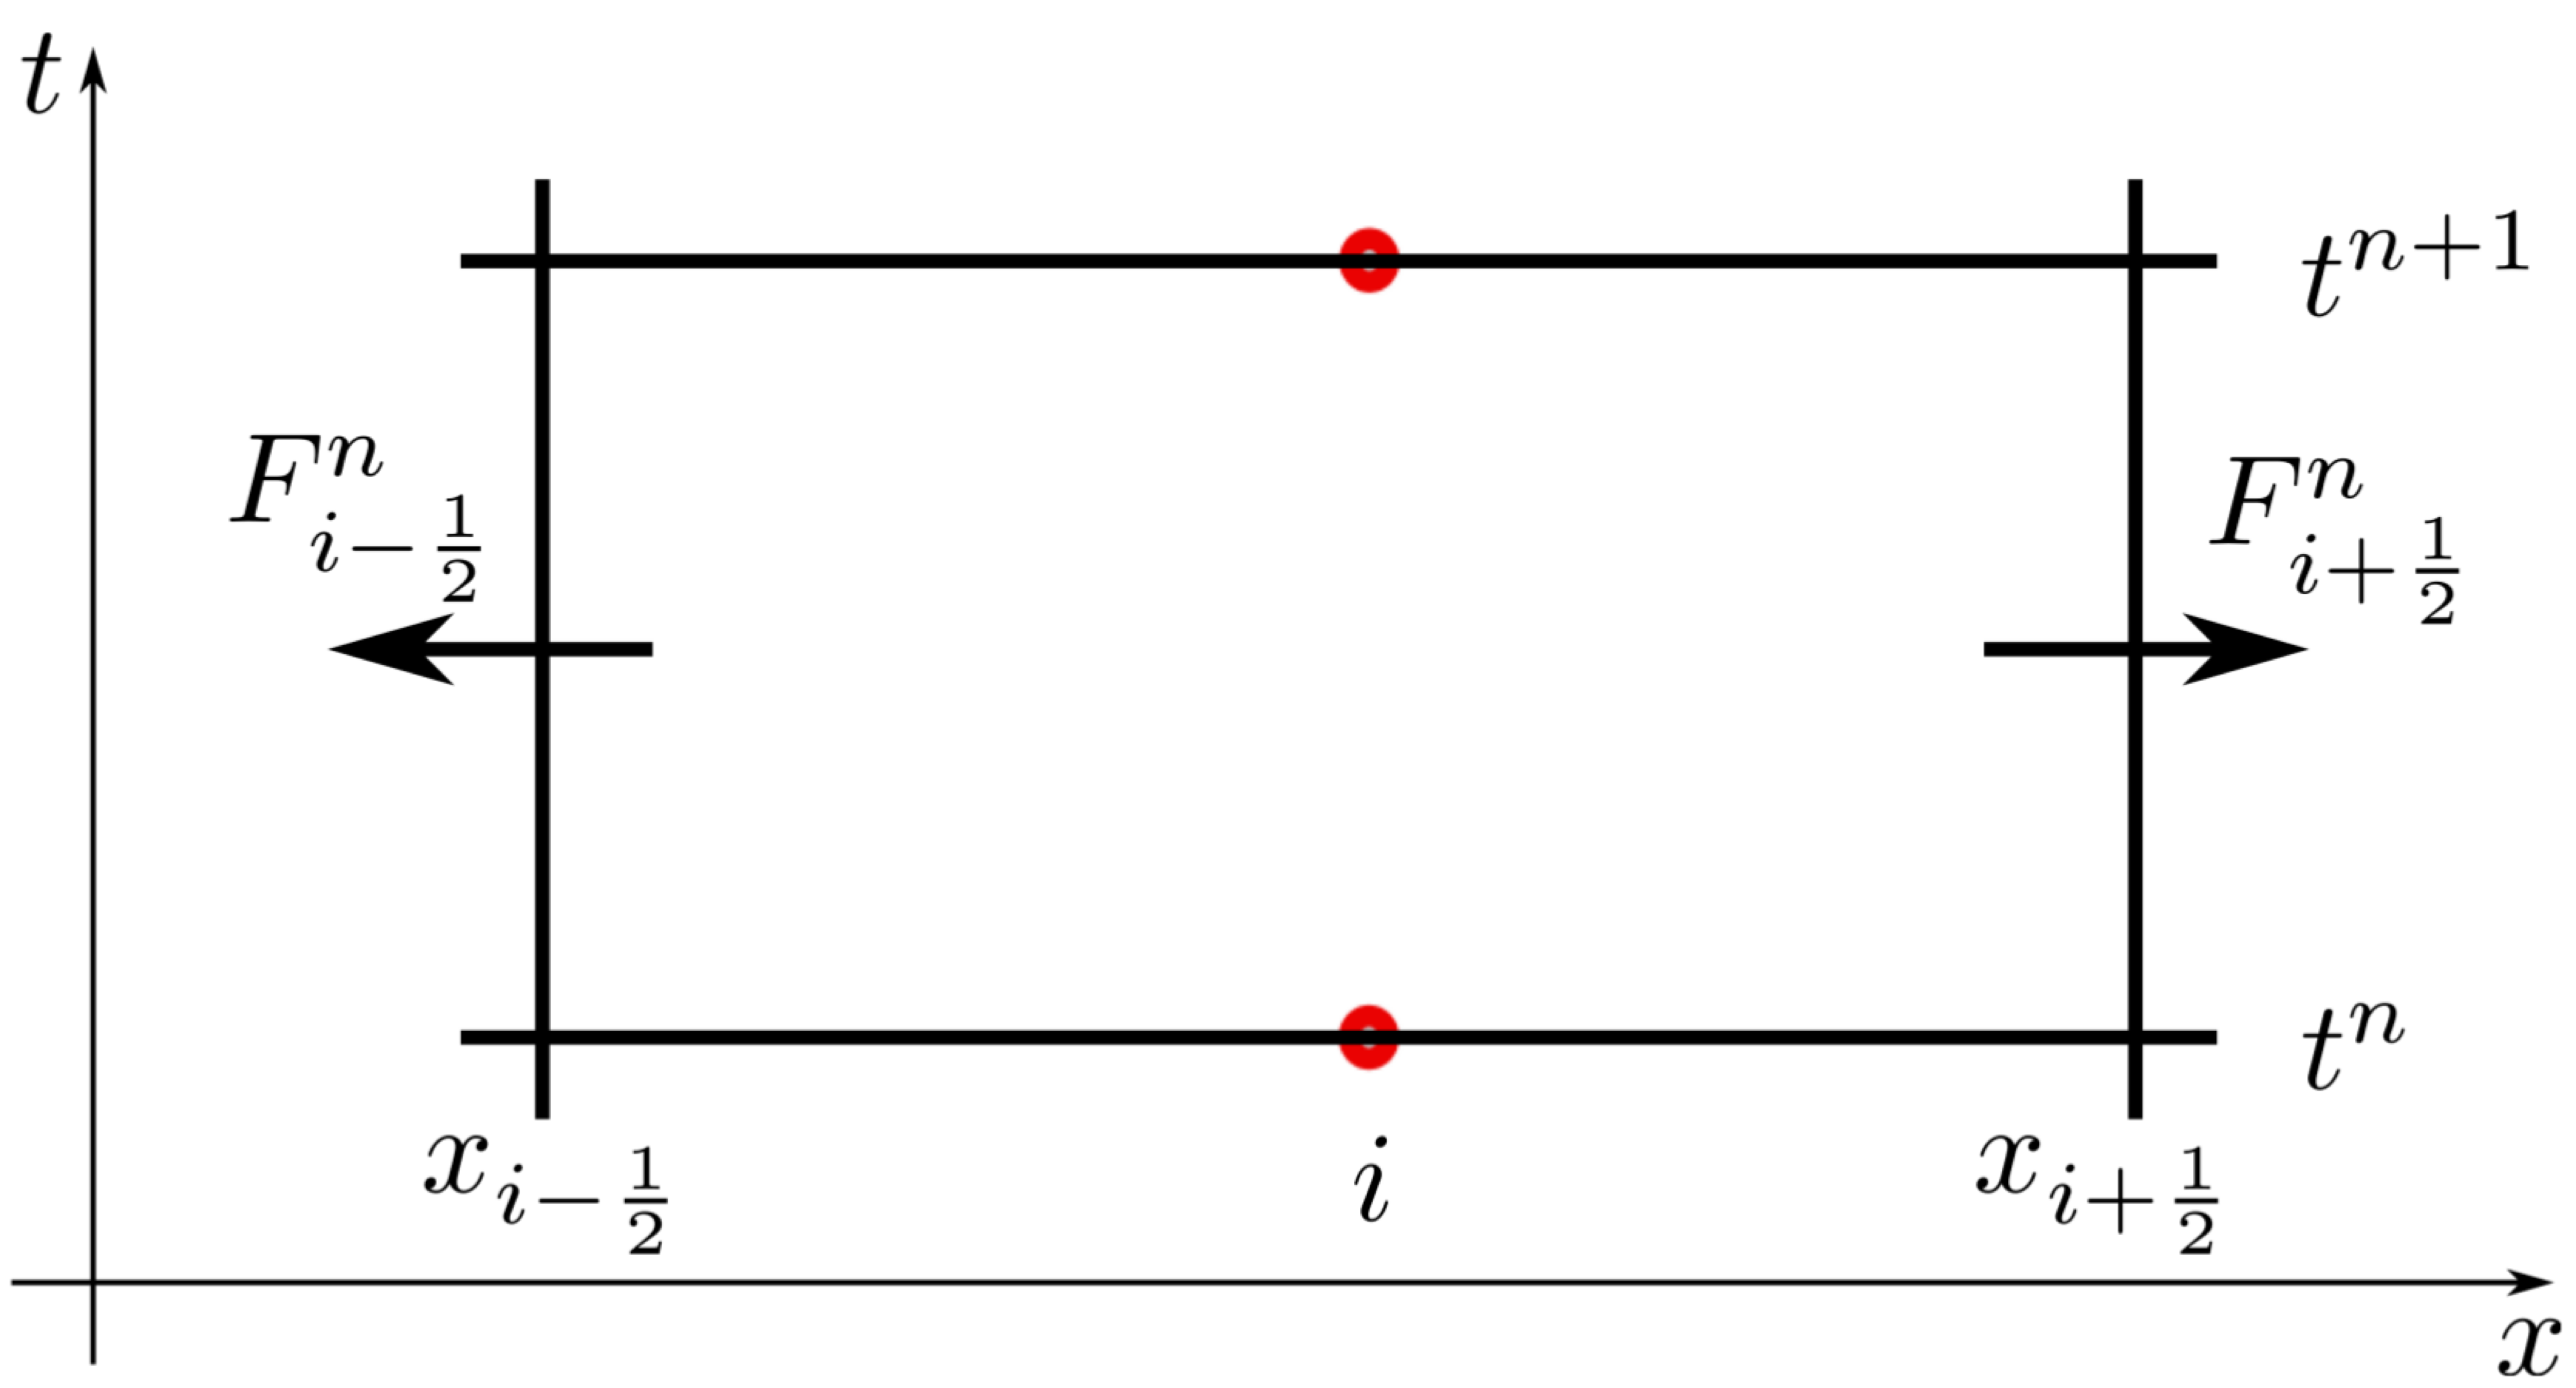
\includegraphics[width=0.5\columnwidth]{Volume di Controllo.png}
    \caption{Volume di controllo}
    \label{fig:Volume di controllo}
\end{figure}
\noindent L'integrale di linea in (\ref{eqn:teorema_Green_app_Riemann}) calcolato lungo il contorno di questo dominio diviene:
\begin{equation}
    \begin{split}
    &\oint F(x,t)dt - U(x,t)dx = \\ &=\int_{t^n}^{t^{n+1}}F\left(x_{i+\frac{1}{2}},t\right)dt+\int_{t^{n+1}}^{t^n}F\left(x_{i-\frac{1}{2}},t\right)dt-\int_{x_{i-\frac{1}{2}}}^{x_{i+\frac{1}{2}}}U\left(x,t^n\right)dx-\int_{x_{i+\frac{1}{2}}}^{x_{i-\frac{1}{2}}}U\left(x,t^{n+1}\right)dx=0 \\
    &=\int_{t^n}^{t^{n+1}}F\left(x_{i+\frac{1}{2}},t\right)dt-\int_{t^n}^{t^{n+1}}F\left(x_{i-\frac{1}{2}},t\right)dt-\int_{x_{i-\frac{1}{2}}}^{x_{i+\frac{1}{2}}}U\left(x,t^n\right)dx+\int_{x_{i-\frac{1}{2}}}^{x_{i+\frac{1}{2}}}U\left(x,t^{n+1}\right)dx=0 \\
    &=\int_{t^n}^{t^{n+1}}F\left(U\left(x_{i+\frac{1}{2}},t\right)\right)dt-\int_{t^n}^{t^{n+1}}F\left(U\left(x_{i-\frac{1}{2}},t\right)\right)dt-\int_{x_{i-\frac{1}{2}}}^{x_{i+\frac{1}{2}}}U\left(x,t^n\right)dx+\int_{x_{i-\frac{1}{2}}}^{x_{i+\frac{1}{2}}}U\left(x,t^{n+1}\right)dx \\ &=0
    \label{eqn:integrale_linea}
    \end{split}
\end{equation}
\noindent ovvero:
\begin{equation}
    \begin{split}
    &\int_{x_{i-\frac{1}{2}}}^{x_{i+\frac{1}{2}}}U\left(x,t^{n+1}\right)dx=-\int_{t^n}^{t^{n+1}}F\left(U\left(x_{i+\frac{1}{2}},t\right)\right)dt+\int_{t^n}^{t^{n+1}}F\left(U\left(x_{i-\frac{1}{2}},t\right)\right)dt+\int_{x_{i-\frac{1}{2}}}^{x_{i+\frac{1}{2}}}U\left(x,t^n\right)dx \\
    &\int_{x_{i-\frac{1}{2}}}^{x_{i+\frac{1}{2}}}U\left(x,t^{n+1}\right)dx=\int_{x_{i-\frac{1}{2}}}^{x_{i+\frac{1}{2}}}U\left(x,t^n\right)dx-\left[\int_{t^n}^{t^{n+1}}F\left(U\left(x_{i+\frac{1}{2}},t\right)\right)dt-\int_{t^n}^{t^{n+1}}F\left(U\left(x_{i-\frac{1}{2}},t\right)\right)dt\right]
    \end{split}
    \label{eqn:?}
\end{equation}
\noindent Il dominio $x \in [0, L], t \in [0, \infty)$ è discretizzato in M volumi finiti $V^{i}_n$, di area $\Delta x \times \Delta t$ (Figura \ref{fig:Dominio di Calcolo}).
\begin{figure}
    \centering
    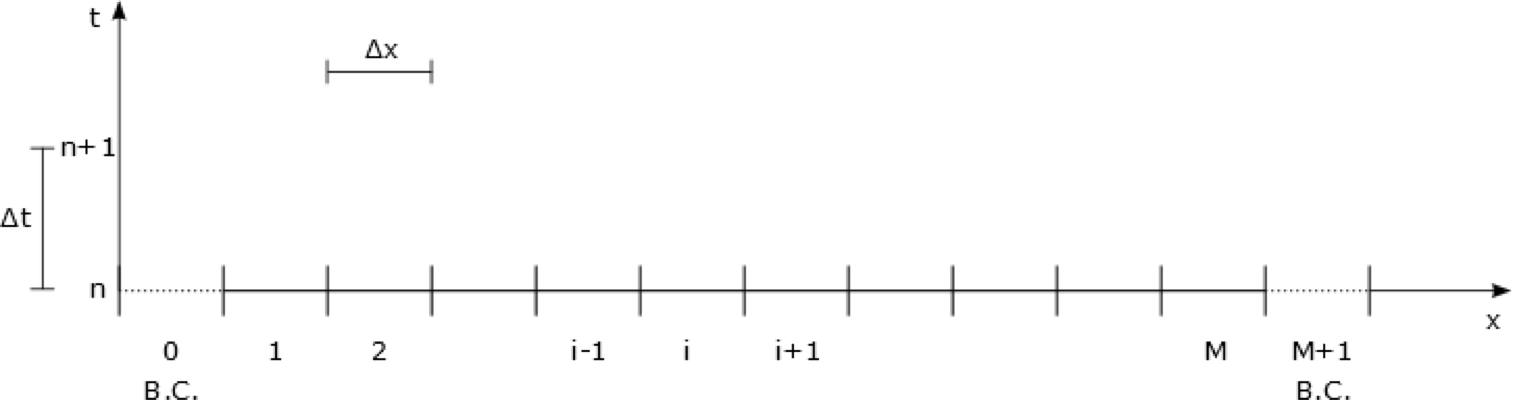
\includegraphics[width=\textwidth]{Dominio di Calcolo.png}
    \caption{Dominio di Calcolo}
    \label{fig:Dominio di Calcolo}
\end{figure}
\noindent Dividendo (\ref{eqn:?}) per $\Delta x$:
\begin{equation}
    \begin{split}
    &\frac{1}{\Delta x}\int_{x_{i-\frac{1}{2}}}^{x_{i+\frac{1}{2}}}U\left(x,t^{n+1}\right)dx= \\ &\frac{1}{\Delta x}\int_{x_{i-\frac{1}{2}}}^{x_{i+\frac{1}{2}}}U\left(x,t^n\right)dx-\frac{1}{\Delta x}\left[\int_{t^n}^{t^{n+1}}F\left(U\left(x_{i+\frac{1}{2}},t\right)\right)dt-\int_{t^n}^{t^{n+1}}F\left(U\left(x_{i-\frac{1}{2}},t\right)\right)dt\right]
    \end{split}
    \label{eqn:?_1/Deltax}
\end{equation}
\noindent Moltiplicando e dividendo per $\Delta t$:
\begin{equation}
    \begin{split}
    &\frac{1}{\Delta x}\int_{x_{i-\frac{1}{2}}}^{x_{i+\frac{1}{2}}}U\left(x,t^{n+1}\right)dx= \\ &\frac{1}{\Delta x}\int_{x_{i-\frac{1}{2}}}^{x_{i+\frac{1}{2}}}U\left(x,t^n\right)dx-\frac{\Delta t}{\Delta x}\left[\frac{1}{\Delta t}\int_{t^n}^{t^{n+1}}F\left(U\left(x_{i+\frac{1}{2}},t\right)\right)dt-\frac{1}{\Delta t}\int_{t^n}^{t^{n+1}}F\left(U\left(x_{i-\frac{1}{2}},t\right)\right)dt\right]
    \end{split}
    \label{eqn:?_Deltat/Deltax}
\end{equation}
Possiamo notare che i termini dell'uguaglianza rappresentano nientemeno che le approssimazioni di $U$ ed $F$:
\begin{equation}
    \begin{split}
    &U = \frac{\partial}{\partial x}\int U dx \approx \frac{\Delta\int U dx}{\Delta x} \\
    &F = \frac{\partial}{\partial t}\int F dt \approx \frac{\Delta\int F dt}{\Delta t}
    \end{split}
\end{equation}
\noindent Considerato l'i-esimo volume di controllo rettangolare $[x_{i-\frac{1}{2}},x_{i+\frac{1}{2}}] \times [t^n,t^{n+1}]$, la discretizzazione di (\ref{eqn:?}) risulta:
\begin{equation}
    U_i^{n+1}=U_i^{n}-\frac{\Delta t}{\Delta x}\left(F_{i+\frac{1}{2}}^n-F_{i-\frac{1}{2}}^n\right)
    \label{eqn:Riemann_discreto}
\end{equation}
\noindent dove:
\begin{align*}
    &U_i^{n}=\frac{1}{\Delta x}\int_{x_{i-\frac{1}{2}}}^{x_{i+\frac{1}{2}}}U\left(x,t^n\right)dx
    &U_i^{n+1}=\frac{1}{\Delta x}\int_{x_{i-\frac{1}{2}}}^{x_{i+\frac{1}{2}}}U\left(x,t^{n+1}\right)dx \\ &F_{i+\frac{1}{2}}^n=\int_{t^n}^{t^{n+1}}F\left(U\left(x_{i+\frac{1}{2}},t\right)\right)dt
    &F_{i-\frac{1}{2}}^n=\int_{t^n}^{t^{n+1}}F\left(U\left(x_{i-\frac{1}{2}},t\right)\right)dt
\end{align*}
\subsubsection{Metodi centrati}
\noindent L'idea alla base della costruzione di soluzioni approssimate per il PVI (\ref{eqn:Riemann}), (\ref{eqn:Riemann_cond_iniziali}) è quella della discretizzazione temporale. Si definisce una sequenza di tempi $0=t_0<t_1<t_2<...$ con un passo fisso $\Delta t>0$ tale che $t_n=n\Delta t$, con $n=0,1,2...$. L'equazione discreta (\ref{eqn:Riemann_discreto}) è usata per determinare  $U^{n+1}(x)$, a patto che sia già conosciuta  $U^{n}(x)$. Consideriamo ora una sequenza di punti spaziali equamente distanti $x_i=i\Delta x$, con $-\infty\leq i \leq+\infty$. La funzione $U^{n}(x)$ può essere rappresentata dai valori che assume nei punti della griglia computazionale $U_i^{n}=U(x_i,t_n)$. Essendo tuttavia la funzione $U(x,t)$ sconosciuta per $x > x_i$, è necessario interpolare $U\left(x_{i-\frac{1}{2}},t_n\right)$ e $U(x_i,t_n)$ al fine di stimare $U\left(x_{i+\frac{1}{2}},t_n\right)$. La maniera in cui i valori di $U^n\left(x_{i-\frac{1}{2}}\right)$ e $U^n(x_i)$ sono interpolati per determinare $U^n\left(x_{i+\frac{1}{2}}\right)$ definisce la classe di metodi numerici di risoluzione che possono essere costruiti:
\begin{itemize}
    \item Metodo di Lax-Friedrichs
    \begin{equation}
        F_{i+\frac{1}{2}}^{LF}=\frac{1}{2}\left[F(U_{i-1}^n)+F(U_i^n)\right]-\frac{\Delta x}{2\Delta t}(U_i^n-U_{i-1}^n)
        \label{eqn:Lax-Friedrichs}
    \end{equation}
    \item Metodo di Lax-Wendroff
        \begin{equation}
        \begin{split}
           &F_{i+\frac{1}{2}}^{LW}=F(U_{i+\frac{1}{2}}^{LW}) \\
           &U_{i+\frac{1}{2}}^{LW}=\frac{1}{2}\left(U_i^n+U_{i+1}^n\right)+\frac{1}{2}\frac{\Delta t}{\Delta x}\left(F_i^n-F_{i+1}^n\right)
        \end{split}
        \label{eqn:Lax-Wendroff}
    \end{equation}
    \item Metodo FORCE (First Order Centered)(Toro E. F. 2001)
    \begin{equation}
        F_{i+\frac{1}{2}}^{TO}=\frac{1}{2}\left[F_{i+\frac{1}{2}}^{LF}+F_{i+\frac{1}{2}}^{LW}\right]
        \label{eqn:FORCE}
        \end{equation}
\end{itemize}
\subsubsection{Metodo di Runge-Kutta}

\subsection{Analisi dei metodi numerici adottati}
\subsubsection{Consistenza e convergenza}
\noindent Per un dato schema numerico, l'errore di troncamento locale $\tau$ è l'errore che si genera pretendendo che la soluzione esatta verifichi lo schema numerico stesso.
Per uno schema unidimensionale, $\tau$ è  funzione del passo di discretizzazione temporale $\Delta t$ e  dell'intervallo di discretizzazione spaziale $\Delta x$. Lo schema numerico si dirà consistente se l'errore di troncamento $\tau(\Delta t, \Delta x)$ tende a zero quando $\Delta t$ e $\Delta x$ tendono a zero (Quarteroni A. 2006).
\subsubsection{Stabilità}
\noindent Molto spesso nel contesto di problemi iperbolici si cercano soluzioni per tempi lunghi (cioè per $T\gg1$). In questi casi è richiesta la forte stabilità dello schema, in quanto essa garantisce che la soluzione numerica sia limitata per ogni valore di $T$. In uno schema alle differenze finite come (\ref{eqn:Riemann_discreto}), il valore di $U_i^{n+1}$ dipende, in generale, soltanto dai valori di $U^{n}_{i-\frac{1}{2}}$, $U^{n}_{i}$ e $U^{n}_{i+\frac{1}{2}}$. Procedendo all'indietro si desume che la soluzione $U_i^{n+1}$ dipenderà solo dai dati iniziali nei punti $x_{i-\frac{1}{2}}$, $x_i$ e $x_{i+\frac{1}{2}}$, vale a dire $x_i\pm\:\textrm{un certo}\:\Delta x$. Fissato un tempo $t$, il luogo dei punti che giacciono sull'asse delle $x$ che influenzano la soluzione al tempo $t+\Delta t$ è chiamato dominio di dipendenza numerico. Condizione necessaria affinché uno schema numerico esplicito della forma (60) sia stabile, è che $U^{n}_{i-\frac{1}{2}}$, $U^{n}_{i}$ e $U^{n}_{i+\frac{1}{2}}$ non cadano mai al di fuori del dominio di dipendenza numerico di $U_i^{n+1}$ (Figura \ref{fig:CFL}). 
\begin{figure}
    \centering
    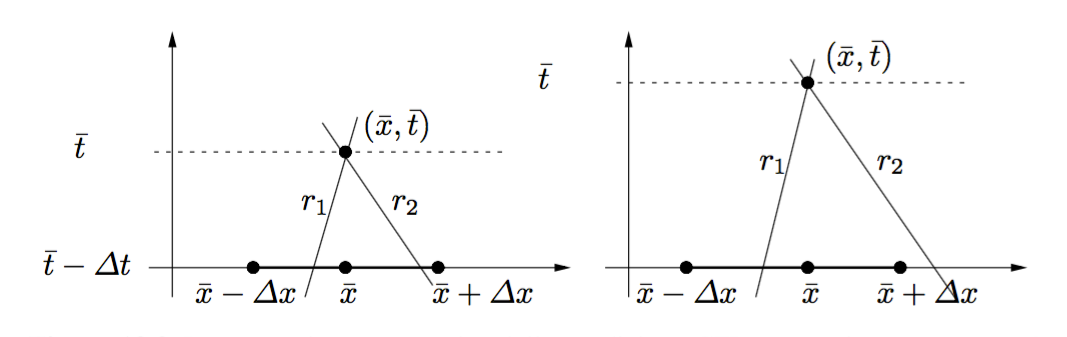
\includegraphics[width=\textwidth]{CFL.png}
    \caption{Interpretazione geometrica della condizione CFL. La condizione CFL è soddisfatta nel caso di sinistra, è violata nel caso di destra}
    \label{fig:CFL}
\end{figure}
\noindent In altre parole, la velocità $\lambda=\frac{dx}{dt}$ con cui ci si sposta lungo una curva caratteristica da $t$ a $t+\Delta t$ deve essere sempre minore della "velocità della griglia di calcolo" $\frac{\Delta x}{\Delta t}$. In formule:
\begin{equation}
    \frac{\lambda}{\Delta x/\Delta t}\leq1
    \label{eqn:Courant}
\end{equation}
\noindent dove:
\begin{itemize}
    \item $\lambda$ è il maggiore autovalore soluzione dell'equazione \ref{eqn:determinante_uguale_zero}.
\end{itemize}
\noindent Il rapporto $\frac{\lambda}{\Delta t/\Delta x}$ rappresenta una quantità adimensionale detta numero di CFL (da Courant, Friedrichs e Lewy) o numero di Courant. La relazione (\ref{eqn:Courant}) si riassume quindi a: 
\begin{equation}
    CFL\leq1
\end{equation}
\noindent dove:
\begin{itemize}
\item $CFL$ è il numero di Courant [$adm$]
\end{itemize}
\noindent  che viene detta condizione CFL. Nella pratica, il numero di CFL viene fissato a 0.9.
Imporre $CFL=0.9$ ci permette di determinare il passo temporale secondo la seguente relazione:
\begin{equation}
    \Delta t=0.9\frac{\Delta x}{\lambda}
\end{equation}
\noindent che deriva direttamente dalla definizione di numero  di CFL.

\subsection{Condizioni iniziali e al contorno adottate}
\begin{itemize}
\item\textbf{Condizioni al contorno di valle}
\begin{itemize}
    \item Condizione trasmissiva
    \begin{equation}
        \begin{cases}
        Y(M+1,t)=Y(M,t)\\
        q(M+1,t)=q(M,t)
        \end{cases}
    \end{equation}
    \item Condizione riflessiva
    \begin{equation}
        \begin{cases}
        Y(M+1,t)=Y(M,t)\\
        q(M+1,t)=-q(M,t)
        \end{cases}
    \end{equation}
\end{itemize}
\item\textbf{Condizioni al contorno di monte}
\begin{itemize}
    \item Condizione trasmissiva
    \begin{equation}
        \begin{cases}
        Y(0,t)=Y(1,t)\\
        q(0,t)=q(1,t)
        \end{cases}
\end{equation}
    \item Condizione riflessiva
    \begin{equation}
        \begin{cases}
        Y(0,t)=Y(1,t)\\
        q(0,t)=-q(1,t)
        \end{cases}
    \end{equation}
\end{itemize}
\end{itemize}
\subsubsection{Condizioni al contorno di monte}
\noindent Note le caratteristiche geometriche ed idrauliche del corso d'acqua, nel caso di corrente localmente veloce si impone:
\begin{equation}
    Y(0,t)=Y(q_0(t))
\end{equation}
\noindent dove:
\begin{itemize}
    \item $Y(q_0(t))$ è il tirante $Y$ [$m$] calcolato a partire dalla portata attraverso l'equazione del moto uniforme
    \item $q_0(t)$ è l'idrogramma di piena [$m^2\cdot s^{-1}$]
\end{itemize}
\noindent Nel caso di corrente localmente lenta, invece, $Y(0,t)$ è calcolato ricorrendo al sistema di equazioni di governo scritto in forma caratteristica (\ref{eqn:forma_caratteristica}) nella seguente maniera:
\begin{itemize}
    \item $q(0,t^{n+1})$ è assegnato (idrogramma di piena)
    \item $Y(0,t^{n+1})$ viene imposto utilizzando l'equazione (\ref{eqn:forma_caratteristica}) associata a $\lambda^-$:
\end{itemize}
\begin{equation}
    \left(-u-\sqrt{gY}\right)\frac{dY}{dt}+\frac{dq}{dt}-gY\left(i_F-j\right)=0
\end{equation}
\begin{figure}
    \centering
    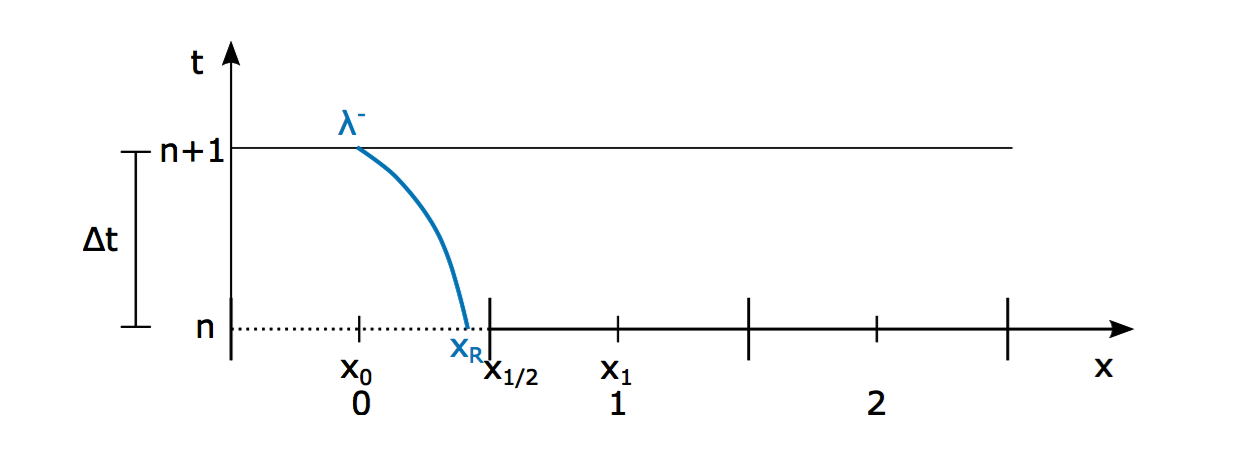
\includegraphics[width=0.7\textwidth]{Piede xR.png}
    \caption{Condizione al contorno di monte}
    \label{fig:piede xR}
\end{figure}



\section{Parte scritta da Marco}
\subsection{Dam Break}
\noindent Per la risoluzione del problema di rottura di una diga si considera, in fase iniziale (t=0), una situazione di integrità della struttura e di stabilità del fluido:

\begin{itemize}
\item A monte 
\begin{equation}
 Y=Y\textsubscript{$0$}, U=0
\end{equation}
\item A valle
\begin{equation}
 Y=0, U=0
\end{equation}
\end{itemize}

\noindent Le ipotesi di partenza prevedono alveo rettangolare largo e l’assenza dell’effetto frizionale, bilanciato da quello gravitazionale.
Nello stesso istante si considera il crollo improvviso della diga e l’inizio del fenomeno di dispersione del fluido, che si propaga nello spazio per mezzo di due onde: una di sommersione verso valle e una di rarefazione verso monte.
Le equazioni caratteristiche son le seguenti:

\begin{equation}
\frac{dx}{dt}=U\pm \sqrt{gY}
\end{equation}

\begin{equation}
U \pm 2\sqrt{gY}=cost
\end{equation}

\noindent Nelle suddette condizioni le celerità con cui si propagano le due onde sono, rispettivamente, $c=2\sqrt{gY\textsubscript{$0$}}$ e $c=-\sqrt{gY}$.
Il tirante della regione di onda semplice viene espresso come
Dall’analisi del fenomeno si può dedurre l’esistenza di un punto di criticità della corrente, corrispondente al luogo di passaggio tra la corrente lenta a monte e veloce a valle. Tale punto si posiziona in corrispondenza della diga ad un’altezza pari a 

\begin{equation}
    Y=\frac{4}{9}Y\textsubscript{$0$}
\end{equation}
\subsection{Modello cinematico}
\noindent Si tratta del modello più semplice per lo studio del fenomeno, caratterizzato da un’equazione dinamica semplificata dai suoi termini inerziali e gravitazionali che la rende di fatto una legge di moto localmente uniforme:
\begin{equation}
\frac{\partial \Omega }{\partial t}+U\frac{\partial Q}{\partial x}=0
\end{equation}
\begin{equation}
Q=C\Omega\sqrt{gR_hi_f}=kY^m
\end{equation}

\noindent La seconda equazione è la cosiddetta scala di deflusso per moto uniforme, legge che lega la portata al tirante; i parametri k ed m, per ipotesi di alveo cilindrico (geometria costante), non sono dipendenti dalla coordinata spaziale.
Il termine di conduttanza C viene espresso con la formula di Gauckler Strickler.\\
I valori di celerità dell’onda di piena si ricavano dalla relazione $\frac{\partial Q}{\partial \Omega}$;
fisicamente il termine corrisponde alla velocità dell’onda, descritta anche come la variazione della portata lungo l’area.
Considerando l’ipotesi di alveo rettangolare largo (area costante), la celerità si può esprimere nel seguente modo:

\begin{equation}
c=\frac{1}{b}\frac{\partial Q}{\partial Y}
\end{equation}

Derivando la portata per il tirante:

\begin{equation} 
c=\frac{1}{b}mkY^{m-1}=\frac{Q}{\Omega}\frac{\Omega}{bY}=mU\frac{Y\textsubscript{$m$}}{Y}
\end{equation}

\noindent Dall’equazione si nota la proporzionalità diretta tra la celerità c e il tirante Y; questo esprime fisicamente una maggiore velocità di propagazione dell’onda all’aumentare del tirante di fluido.
All’interno del fenomeno la relazione comporta che il picco della piena si muove più velocemente rispetto agli altri punti, generando una progressiva deformazione temporale dell’onda che si esaurisce nel suo frangimento finale.
Questo aspetto fenomenologico non è contemplato nel caso reale, ma è previsto all’interno del modello a causa delle grosse semplificazioni che costringono all’uso di un’equazione differenziale di primo grado con un’unica condizione imposta a monte, perciò priva di condizioni a valle.

\subsection{Modello parabolico}
\noindent A differenza del precedente modello, quello parabolico risulta più complesso in quanto trascura solamente il termine inerziale:

\begin{equation}
\frac{\partial \Omega }{\partial t}+U\frac{\partial Q}{\partial x}=0
\end{equation}
\begin{equation}
\frac{\partial Y }{\partial x}=if-j
\end{equation}

\noindent In questo caso l’equazione della portata tiene conto del termine frizionale:

\begin{equation}
    Q=C\Omega\sqrt{gR\textsubscript{$H$}(if-\frac{\partial Y}{\partial x}})
\end{equation}

\noindent Inserendo tale relazione nell’equazione della continuità, si ottiene la seguente equazione alle derivate parziali di secondo ordine:

\begin{equation}
\frac{\partial Y}{\partial t}+c\frac{\partial Y}{\partial x}=D\frac{\partial Y^2}{\partial x^2}
\end{equation}

\noindent Al termine $D=\frac{Q}{2bj}$, coefficiente di diffusione, si lega l’incremento o l’attenuazione dell’onda.
Considerando una sezione fissata, è possibile plottare graficamente l’andamento del tirante dell’onda in relazione alla portata caratteristica; la forma che ne consegue, conosciuta come cappio di piena, rappresenta in maniera ottimale la differenza tra il massimo locale dell’onda ($\frac{\partial Y}{\partial x} = 0$) e il colmo di piena ($Q=Qmax$), associati a due punti diversi dell’evento ondoso.

\subsection{Condizioni iniziali e al contorno}
\noindent La risoluzione di un problema di equazioni differenziali necessita della definizione di un certo numero di condizioni al bordo, sia iniziali che al contorno, in base al grado dell’equazione.
Nei casi trattati le condizioni iniziali ($t=0$), ossia i valori delle incognite all’instante iniziale, sono le seguenti:

\begin{itemize}
\item Onda di piena: portata unitaria e tirante di moto uniforme
\item Dam Break: tirante unitario a sx della diga, tirante nullo a dx, velocità nulla in entrambi i lati
\end{itemize}

\noindent Si definisce inoltre il dominio di calcolo, dato dal seguente range di coordinate spaziali:
Le condizioni al contorno, invece, ossia i valori delle variabili in determinati punti del dominio per qualsiasi istante, sono definite dal comportamento delle onde ai bordi del dominio, le quali in genere rispettano i seguenti principi:

\begin{itemize}
\item Trasmissività: le celle ai bordi del dominio di calcolo assumono il valore e il segno della cella adiacente
\item Riflessività: l’onda di piena, a contatto con parete riflettente, viene respinta e inverte il suo verso di moto
\end{itemize}

\noindent Le condizioni, rispettivamente trasmissiva e riflessiva, vengono espresse analiticamente nel seguente modo:
\begin{itemize}
\item A monte: 
\begin{equation}
\begin{cases}
    Y(0,t)=Y(1,t)\\
    q(0,t)=q(1,t)
    \end{cases}
    \begin{cases}
    Y(0,t)=Y(1,t)\\
    q(0,t)=-q(1,t)
    \end{cases}
\end{equation}
\item A valle:
\begin{equation}
\begin{cases}
    Y(M+1,t)=Y(M,t)\\
    q(M+1,t)=q(M,t)
    \end{cases}
    \begin{cases}
    Y(M+1,t)=Y(M,t)\\
    q(M+1,t)=-q(M,t)
    \end{cases}
\end{equation}
\end{itemize}

\subsection{Notazione vettoriale}
\noindent La trattazione del problema riportata in scrittura vettoriale si esprime tramite la definizione dei seguenti vettori:
\begin{itemize}
    \item Incognite:
    \begin{equation}
        U=\begin{pmatrix}
            Y\\
            q
        \end{pmatrix}
    \end{equation}
    \item Flusso:
    \begin{equation}
        F=\begin{pmatrix}
            q\\
            Q\frac{q^2}{Y}+g\frac{Y^2}{2}
        \end{pmatrix}
    \end{equation}
    \item Sorgente:
    \begin{equation}
        F=\begin{pmatrix}
            0\\
            gY(if-j)
        \end{pmatrix}
    \end{equation}
\end{itemize}
L’equazione generale che racchiude, in forma vettoriale, le espressioni analizzate in precedenza diventa la seguente:
\begin{equation}
    \frac{\partial U}{\partial t}+\frac{\partial F(U)}{\partial x}=S(U)
\end{equation}

\noindent con il secondo termine esprimibile in funzione del primo tramite l’uso del termine jacobiano del sistema J(U):

\begin{equation}
    \frac{\partial F(U)}{\partial x}=J(U)\frac{\partial U}{\partial x}
\end{equation}

\begin{equation}
J(U)=\begin{bmatrix}
0 & 1\\
-\frac{q^2}{Y^2}+gY & \frac{2g}{Y}
\end{bmatrix}
\end{equation}
Un sistema alle derivate parziale del primo ordine ammette un’unica soluzione se esso è iperbolico, cioè la matrice J(U) possiede autovalori reali e linearmente indipendenti.
Una volta risolto tale problema, le radici ottenute come soluzione del polinomio caratteristico della matrice sono l’espressione delle curve caratteristiche che descrivono il moto di propagazione dell’onda, lungo le quali le seguenti espressioni rimangono costanti:

\begin{equation}
    c^{\pm}=u\pm 2\sqrt{gY}=cost
\end{equation}

\subsection{Metodo ai volumi finiti}
\noindent Per la risoluzione del sistema di equazioni vettoriali descritto in precedenza ci si avvale del metodo ai volumi finiti.
L’approccio modellistico prevede la suddivisione del dominio di calcolo in una mesh computazionale di risoluzione variabile, all’interno della quale viene approssimata la media integrale delle equazioni trattate, soddisfando al contempo entrambi i principi di conservazione. Le variabili, pertanto, vengono derivate come differenze discrete tra valori di due celle diverse adiacenti.
Innanzitutto il dominio di controllo viene discretizzato in M celle  di forma rettangolare, o volumi finiti, definiti nel piano (x,t) come:

\begin{equation}
    V^{i}_n=[x_{1-\frac{1}{2}},x_{i+\frac{1}{2}}]\times[t^n,t^{n+1}]
\end{equation}

\noindent La cella i-esima perciò ha dimensione $\Delta x\Delta t$.

\noindent Il sistema scritto in forma vettoriale

\begin{equation}
    \frac{\partial U}{\partial t}+\frac{\partial F}{\partial x}=S(U)
\end{equation}

\noindent può esser scritto in forma integrale nel seguente modo:

\begin{equation}
    \int Udx+F(U)dt=0
\end{equation}

\noindent Per ogni cella del dominio si ricava il valore medio del vettore incognite, assunto come costante all’interno della cella. Dalla discretizzazione nel volume infinitesimo si ottiene:

\begin{equation}
    U^{n+1}\textsubscript{$i$}= U^{n}\textsubscript{$i$}-\frac{\Delta t}{\Delta x}(F\textsubscript{$1+\frac{1}{2}$}-F\textsubscript{$1-\frac{1}{2}$})
\end{equation}

\noindent Le variabili conservate indefinite, rappresentate dal termine $F\textsubscript{$1+\frac{1}{2}$}$, si possono determinare con diversi schemi numerici:
\begin{itemize}
    \item Lax-Friedrichs 
    \begin{equation}
        f\textsubscript{$1+\frac{1}{2}$}=\frac{1}{2}(f(q^n\textsubscript{$i+1$})+f(q^n\textsubscript{$i$}))-\frac{\Delta x}{2\Delta t}(q^n\textsubscript{$i+1$}+q^n\textsubscript{$i$})
    \end{equation}
    \item Lax-Wendroff 
     \begin{equation}
        f\textsubscript{$1+\frac{1}{2}$}=f(\frac{1}{2}(q^n\textsubscript{$i+1$})+f(q^n\textsubscript{$i$}))-\frac{\Delta x}{2\Delta t}(q^n\textsubscript{$i+1$}+q^n\textsubscript{$i$})
    \end{equation}
    \item Force
     \begin{equation}
      f\textsubscript{$1-\frac{1}{2}$}=\frac{1}{2}(F^{LF}\textsubscript{$i-\frac{1}{2}$}+F^{LW}\textsubscript{$i-\frac{1}{2}$})
    \end{equation}
\end{itemize}

\noindent Lo svolgimento dell’equazione vettoriale del problema si divide in due procedure di natura differente, aventi entrambe la medesima condizione iniziale: una legata alla risoluzione di una PDE con risultato nullo, che fornisce un termine finale puramente convettivo, e un’altra legata alla risoluzione di una ODE con risultato pari al termine sorgente.
La condizione di stabilità per gli schemi elencati è legata al numero di Courant (CFL)

\begin{equation}
    CFL=\lambda\frac{\Delta t}{\Delta x}
\end{equation}

\noindent che rappresenta il rapporto tra la velocità di flusso e la velocità della griglia di calcolo. Per la stabilità e l’accuratezza del metodo è necessario che CFL<1, perciò il numero viene fissato a 0,9.
La stabilità dei metodi si lega quindi alle dimensioni del passo temporale, il quale può assumere come massimo valore

\begin{equation}
    \Delta t=CFL\frac{\Delta x}{\lambda\textsubscript{$max$}}
\end{equation}
con $\lambda\textsubscript{$max$}$ autovalore maggiore.

\newpage

\section {Risultati}

\noindent La rappresentazione dei casi studio precedentemente analizzati è stata condotta tramite implementazione di un codice Python che acquisisca i dati di input (geometrie, condizioni iniziali e al contorno, ecc..), rielabori le equazioni indicate e fornisca in output le immagini riportate nel seguente paragrafo.

\subsection{Crollo della diga}

\noindent Graficamente la simulazione del crollo improvviso della diga ci riporta un'immagine in cui viene riprodotto il livello di tirante sviluppatosi all'interno del dominio spaziale in seguito alla rimozione della parete di contenimento. 
In seguito al fenomeno di crollo, la condizione riflessiva posta a valle del serbatoio, in cui il tirante è costante, viene meno.
Dal momento di rottura della diga, l'acqua contenuta dalla diga si riversa nello spazio restante, con un aumento progressivo del livello di tirante verso valle e una diminuzione altrettanto progressiva verso monte. Osservando i singoli profili di corrente generatisi per ogni istante di simulazione, si nota che essi intersecano la quota di tirante critica, posta in corrispondenza della diga, il quale valore è il seguente:

\begin{equation}
    Y_c=\frac{4}{9}Y_0
\end{equation}

\noindent con $Y_0$ livello di tirante a monte della diga.

\noindent I profili di tirante del flusso d'acqua in propagazione si descrivono analiticamente, punto per punto, tramite le curve caratteristiche della corrente, le quali, all'interno di un piano orario $x-t$, descrivono un ventaglio di soluzioni che assumono valori negativi verso monte e positivi verso valle. Perciò i profili di corrente a valle della diga vengono descritti da curve caratteristiche positive, dette \textit{onde di sommersione}, mentre quelle a monte da curve caratteristiche negative, dette \textit{onde di rarefazione}.\\
Di seguito si riportano le formule generali delle due onde, rispettivamente di sommersione e di rarefazione:

\begin{align*}
    &c^-=2\sqrt{gY_0}
    &c^-=-\sqrt{gY_0}
\end{align*}


\begin{figure} [H]
    \centering
    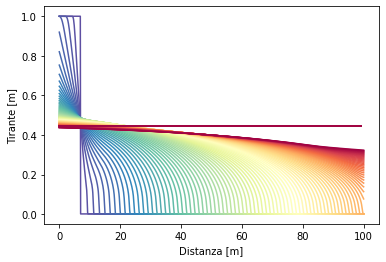
\includegraphics[scale=0.95]{Diga.png}
    \caption{Andamento del tirante in seguito al crollo della diga}
    \label{fig:diga}
\end{figure}

\subsection{Onda di piena}

\noindent Nel caso seguente il grafico riporta l'onda di piena simulata lungo l'ipotetica asta fluviale di lunghezza preimpostata. Il dominio spaziale risulta di diversi ordini di grandezza maggiore rispetto al caso del crollo della diga, per via delle grandi distanze di cui necessita il fenomeno per manifestarsi in maniera apprezzabile.\\
Dal grafico è possibile osservare la conformazione dell'onda di piena all'ultimo istante, con la presenza di un picco assimmetrico e un fronte molto più ripido della coda. Tale proprietà sono riscontrabili in un'onda già progredita nello spazio, e sono dovute al differente sviluppo temporale delle caratteristiche nel caso si tratti di onda positiva ($\frac{\partial Y}{\partial x}<0$) o negativa ($\frac{\partial Y}{\partial x}>0$): nel primo caso le traiettorie delle caratteristiche tendono a convergere, collocando punti con diversi tiranti e velocità sempre più vicini nello spazio, viceversa per le caratteristiche negative che tendono a divergere. Tuttavia, nel caso analizzato, la forma dell'onda perde progressivamente ripidità per via dell'effetto attenuatorio esercitato dall'attrito lungo il percorso, che riduce il picco e la pendenza dei tratti ascendente/discendente.

\begin{figure} [H]
    \centering
    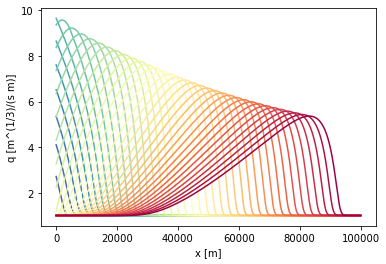
\includegraphics{Onda.png}
    \caption{Andamento del tirante in seguito al crollo della diga}
    \label{fig:onda}
\end{figure}

\noindent La variazione progressiva della portata al passaggio dell'onda, in virtù della natura non stazionaria del fenomeno, trova riscontro grafico nel cosiddetto \textit{cappio di piena} \ref{fig:cappio}. \\ L'andamento della figura, se letta in senso antiorario, ci indica che la fase ascendente dell'onda di piena corrisponde ad un aumento della portata transitante, mentre la fase discendente si accompagna ad un aumento del tirante, in riferimento alla scala di moto uniforme. In particolare, l'andamento del valore delle proprietà della corrente è caratterizzato dai i seguenti passaggi, descritti in ordine temporale:
\begin{itemize}
    \item punto di massimo locale della velocità, tangente alla retta $U=cost$ ($\frac{\partial U}{\partial t}=0$)
    \item punto di massimo della portata ($\frac{\partial Q}{\partial t}=0$)
    \item punto di colmo della piena ($\frac{\partial Y}{\partial t}=0$)
    \item punto di massimo locale della profondità, tangente alla scala di deflusso ($\frac{\partial Y}{\partial x}$=0)
\end{itemize}


\begin{figure} [H]
    \centering
    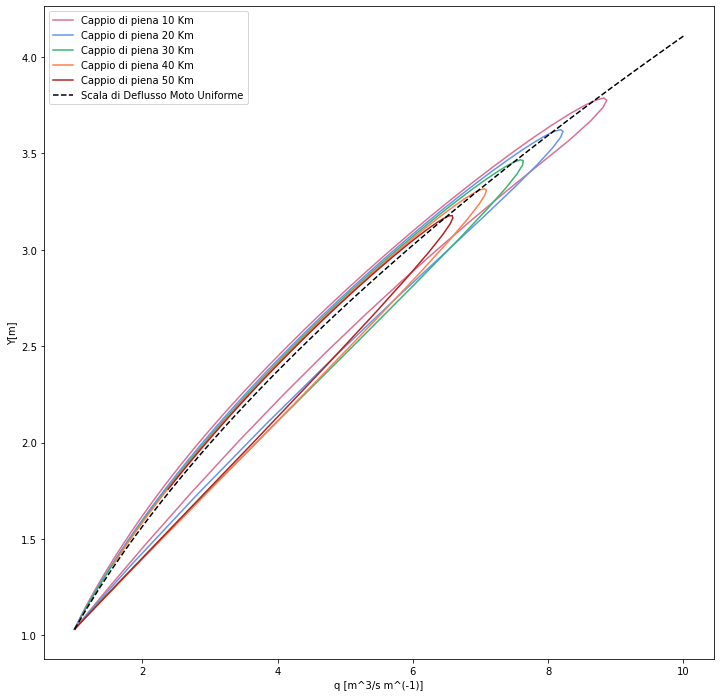
\includegraphics[scale=0.5,width=18cm]{Cappio.png}
    \caption{Andamento del tirante in seguito al crollo della diga}
    \label{fig:cappio}
\end{figure}

\noindent Dalla forma del cappio di piena, in particolare dalla sua eccentricità che regola la distanza dei punti caratteristici dalla scala di deflusso dell'alveo, si può dedurre se la figura si riferisca ad un'onda di piena più o meno accentuata.
Un'analisi qualitativa del grafico ci mostra come i cappi delle onde più brevi abbiano una maggiore apertura, segno del fatto che le variazioni di portata e di tirante rispetto alla scala di deflusso sono maggiori. Questo è indice di come le onde tendano ad attenuarsi progressivamente con il loro sviluppo e ad appiattirsi lungo l'alveo fluviale.

\newpage
\begin{thebibliography}{}
\bibitem{Ben-Artzi M., Falcovitz J. 2003}
Ben-Artzi M., Falcovitz J. (2003) \textit{Generalized Riemann Problems in Computational Fluid Dynamics}. Cambridge University Press
\bibitem{Courant R., Friedrichs K. O. 1977}
Courant R., Friedrichs K. O. (1977) \textit{Supersonic Flow and Shock Waves}. Springer-Verlag, New York Heidelberg Berlin
\bibitem{Pagani C. D., Salsa S. 2016}
Pagani C. D., Salsa S. (2016) \textit{Analisi Matematica 2}. Zanichelli, Bologna
\bibitem{Quarteroni A. 2006}
Quarteroni A. (2006) \textit{Modellistica numerica per problemi differenziali}. Springer-Verlag Italia, Milano
\bibitem{Salsa S. 2016}
Salsa S. (2016) \textit{Equazioni a Derivate Parziali. Metodi, Modelli e Applicazioni}. Springer-Verlag Italia, Milano
\bibitem{Toro E. F. 2001}
Toro E. F. (2001) \textit{Shock-Capturing Methods for Free-Surface Shallow Flows}. John Wiley $\And$ Sons, LTD, Chichester New York Weinheim Brisbane Singapore Toronto 
\end{thebibliography}


\end{document}
